\chapter{La storia di Internet}
Questo capitolo vuole mostrare come Internet sia evoluta da una rete privata a una rete globale in meno di quarant'anni.

\section{La storia iniziale}
Prima del 1960 esistevano già alcune reti di telecomunicazione, come le reti telegrafiche e le reti telefoniche. Queste reti erano adatte a un tipo di comunicazione a velocità costante: era necessario stabilire una connessione fra due utenti prima di poter trasmettere il messaggio codificato (telegrafo) o la voce (telefonia). Una rete di computer, invece, deve essere in grado di gestire traffico bursty (a raffica), ovvero dati trasmessi a varie velocità in tempi differenti. Il mondo attendeva l'invenzione delle reti a commutazione di pacchetto.

La teoria della commutazione di pacchetto per il traffico bursty venne introdotta per la prima volta da Leonard Kleinrock nel 1961 al MIT. Contemporaneamente altri due ricercatori, Paul Baran al Rand Institute e Donald Davies al National Physical Laboratory in Inghilterra pubblicarono alcuni articoli sulle reti a commutazione di pacchetto.

\section{ARPANET}
A metà degli anni '60 i calcolatori centrali dei centri di ricerca erano dei dispositivi a sé stanti. Calcolatori prodotti da industrie diverse non erano in grado di comunicare tra loro. L'Advanced Research Projects Agency (ARPA) del Department of Defense (DOD) era alla ricerca di un metodo per connettere diversi calcolatori, in modo che i ricercatori finanziati con i suoi fondi potessero facilmente condividere i risultati del loro lavoro, riducendo così i costi ed evitando di duplicare gli sforzi.

Nel 1967, a un incontro dell'Association for Computing Machinery (ACM), I'ARPA presentò le sue idee per ARPANET, una piccola rete di calcolatori connessi tra loro. L'idea di base era la seguente: ogni calcolatore sarebbe stato collegato a una macchina dedicata, chiamata Interface Message Processor (IMP). Gli IMP, a loro volta, sarebbero stati collegati tra loro. Ogni IMP doveva essere capace di comunicare con gli altri IMP e con il calcolatore host a esso collegato.

Nel 1969 ARPANET divenne una realtà. I quattro nodi costituiti dalla University of California a Los Angeles (UCLA), dalla University of California a Santa Barbara (UCSB), dallo Standford Research Institute (SRI) e dalla University of Utah, furono collegati attraverso gli IMP e divennero una rete. Il software che realizzava la comunicazione tra i vari calcolatori host fu chiamato Network Control Protocol (NCP).

\section{Nascita della rete Internet}
Nel 1972 Vint Cerf e Bob Kahn, entrambi parte del nucleo del gruppo ARPANET, collaborarono a ciò che chiamarono l'Internetting Project. Il loro scopo era quello di collegare diverse reti in modo che un host di una delle reti potesse comunicare con un altro host di un'altra rete. I problemi da risolvere furono numerosi: dimensione dei pacchetti, interfacce e frequenze di trasmissione diverse, ma anche differenti requisiti di attendibilità.

\section{Internet oggi}
Siamo tutti testimoni della rapidissima evoluzione sia dell'infrastruttura che delle applicazioni di Internet, divenuta oggi una rete che fornisce servizi a livello mondiale. L'incessante sviluppo di nuove applicazioni è il motivo principale della sua diffusione.

Gli anni '90 hanno conosciuto un'esplosione delle applicazioni basate sul World Wide Web (WWW), inventato al CERN da Tim Berners-Lee. Questa invenzione ha aperto Internet alle applicazioni commerciali.

I recenti sviluppi nelle applicazioni multimediali come il Voice Over IP (telefonia su Internet), il video over IP (Skype), la condivisione di video (YouTube) e la televisione su Internet (PPLive) hanno moltiplicato il numero di utenti e il tempo che questi spendono sulla rete.

Le applicazioni di rete peer-to-peer costituiscono un nuovo settore con notevoli potenzialità di sviluppo.

\section{Gli standard della rete Internet}
Uno standard Internet è una specifica che è stata rigorosamente esaminata e controllata, utile e accettata da chi utilizza la rete Internet. È un insieme di regole formalizzate che devono necessariamente essere seguite. Esiste una procedura rigorosa attraverso la quale una specifica diviene uno standard Internet. Il primo stadio di una specifica è quello di bozza Internet (Internet draft). Una bozza Internet è un documento preliminare senza alcuno status ufficiale, la cui vita media è dell'ordine di sei mesi. Su suggerimento delle autorità che regolano la rete Internet una bozza può essere pubblicata come Request for Comments (RFC, richiesta di commenti). Una RFC attraversa, durante la sua vita, sei diversi stadi o livelli di maturità: proposta di standard, bozza di standard, standard Internet, livello storico, sperimentale e informativo.

\begin{figure}[ht]
    \centering
    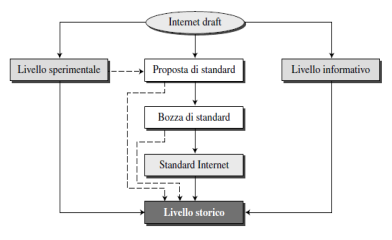
\includegraphics[width=9cm]{images/amministrazione-internet.PNG}
    \caption{Studi di maturazione di una RFC}
    \label{fig:RFC}
\end{figure}

\section{Amministrazione della rete Internet}
La rete Internet, nata sostanzialmente nel mondo della ricerca, si è ampiamente sviluppata e ha raggiunto una base di utenti molto vasta con significative attività commerciali. Numerosi gruppi che coordinano aspetti diversi della rete Internet hanno guidato la sua crescita e il suo sviluppo. Tra questi troviamo: Internet Society (ISOC), Internet Architecture Board (IAB), Internet Engineering Task Force (IETF), Internet Assigned Numbers Authority (IANA) e Internet Corporation for Assigned Names and Numbers (ICANN), Network Information Center (NIC).